\chapter{Theory of Zero-Shot Classification}
\label{appendix:zsc-theory}

This appendix elaborates on zero-shot classification (ZSC), which is used in this system to infer thematic categories for books. Unlike traditional classification methods, ZSC does not require labeled training data for each class. Instead, it relies on a language model’s ability to understand and reason about class labels as natural language.

\section{What is Zero-Shot Classification?}
Traditional classification models require supervised training data — examples of each class to learn from. Zero-shot classification removes this constraint. A model trained on natural language inference (NLI) is reused for classification by rephrasing the task as a premise–hypothesis pair.

\begin{quote}
\textbf{Premise:} “This book is about elves and ancient magic.” \\
\textbf{Hypothesis:} “This text is about fantasy.”
\end{quote}

The model estimates the probability that the hypothesis is entailed by the premise. If high, the label (“fantasy”) is considered appropriate.

\section{Model Foundations}
This project uses \texttt{facebook/bart-large-mnli}, a transformer model fine-tuned on the MultiNLI corpus~\parencite{williams2018broad}. The model performs classification by computing entailment scores between the input and each label reformulated as a natural sentence.

\subsection*{Architecture Overview}
\begin{figure}[H]
\centering
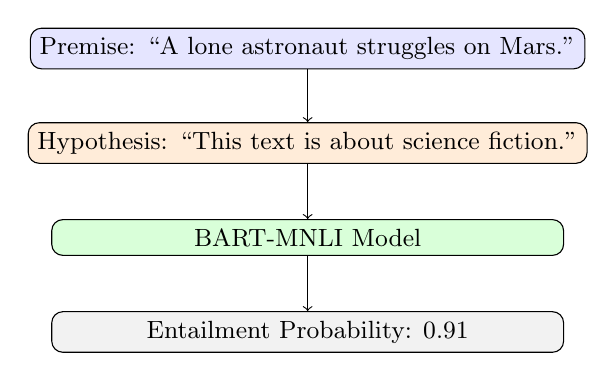
\begin{tikzpicture}[node distance=1.2cm, every node/.style={font=\small}]
    \node (premise) [draw, fill=blue!10, minimum width=6.5cm, rounded corners] {Premise: “A lone astronaut struggles on Mars.”};
    \node (hypo) [below of=premise, draw, fill=orange!15, minimum width=6.5cm, rounded corners] {Hypothesis: “This text is about science fiction.”};
    \node (model) [below of=hypo, draw, fill=green!15, minimum width=6.5cm, rounded corners] {BART-MNLI Model};
    \node (output) [below of=model, draw, fill=gray!10, minimum width=6.5cm, rounded corners] {Entailment Probability: 0.91};

    \draw[->] (premise) -- (hypo);
    \draw[->] (hypo) -- (model);
    \draw[->] (model) -- (output);
\end{tikzpicture}
\caption{Zero-shot classification via textual entailment}
\end{figure}

\section{How It Works in Practice}
Given a book description and a list of candidate genres (e.g., “fantasy”, “science fiction”, “romance”), each label is evaluated independently as a hypothesis. Labels with high entailment scores are retained.

This approach enables:
\begin{itemize}
    \item Multi-label classification: multiple genres can apply
    \item Dynamic label sets: new genres can be introduced without retraining
    \item Minimal supervision: no need for annotated datasets
\end{itemize}

\section{Confidence Thresholding}
The model returns a confidence score for each label. Labels below a threshold (e.g., 0.4) are discarded to reduce noise. Labels just below the threshold may be added through fallback keyword rules.

\section{Fallback Strategies}
To improve coverage when ZSC fails, a rule-based system checks for genre-specific keywords in the description or title. This hybrid approach balances model generalization with deterministic recall.

\section{Limitations}
\begin{itemize}
    \item \textbf{Surface sensitivity:} ZSC may be confused by subtle phrasing
    \item \textbf{High compute cost:} Each label requires a full model pass
    \item \textbf{Bias leakage:} Pretrained models may carry genre biases
\end{itemize}

\section{Conclusion}
Zero-shot classification enables genre inference without labeled examples, making it ideal for low-resource, flexible systems. By treating labels as hypotheses, it leverages the general reasoning ability of transformer models — aligning well with the offline and adaptable design goals of this project.
